\begin{frame}{Summary}
\begin{itemize}
\item The picture revealed by our current results broadly agrees well with that
      of~\cite{ZannaPreprint}, despite the current model being twenty four times
      the temporal resolution, and three times the lateral resolution.
%\item However each year of data does not fully sample the distribution
       (I mean that there can't be the expected fractional number of storms
        in a location in a year), but there may be ways around this.
\item As the coast is a self-similar fractal~\cite{mandelbrot1967long, richardson1961problem},
      it is unclear which length scale to average over to find summary statistics
      for a point on the coast. A reasonable solution would be to give the
      regression algorithm a number of these, and make it decide what is relevant.
\end{itemize}

\end{frame}

\begin{frame}{Current Priorities}
\begin{itemize}
\item Refine measure of the responsiveness  (storm efficiency in~\cite{ZannaPreprint})
      of a coastline unit to a wind stress event.
\item Try to untangle the contribution of
	    convexity, and bathymetry to the responsiveness.
\end{itemize}
\end{frame}

\begin{frame}{Thank you for listening!}
      \begin{minipage}{1.1\textwidth}
   \hspace{-20pt}\begin{minipage}{0.45\textwidth}
   \textbf{Resources Used:}
   \begin{itemize}
\item \texttt{matplotlib}~\cite{Hunter:2007} for original figures,
\item WebPlotDigitiser~\cite{WebPlotDigitiser} for data extraction,
\item Mathpix~\cite{mathpix} for maths extraction,
\item sci-kit-learn~\cite{scikit-learn}  for ML,
\item \texttt{cmocean}~\cite{thyng2016true}
for cmaps,
\item \texttt{numba.jit}~\cite{lam2015numba} for speed,
\item \texttt{uncertainties}~\cite{lebigot2010uncertainties} for error propogation,
\item \texttt{xarray}~\cite{hoyer2017xarray} for ND~data.
\end{itemize}
    \end{minipage}\hspace{10pt}
      \begin{minipage}{0.50\textwidth}
    \begin{figure}
            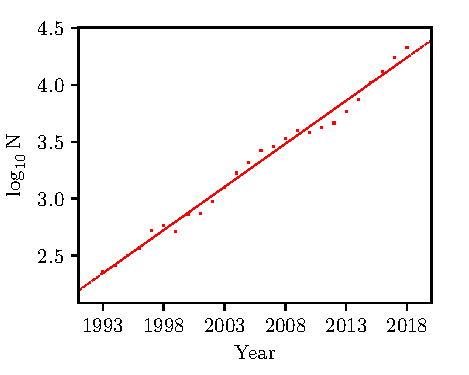
\includegraphics[width=1\linewidth]{images/example-images/Compared_O2.pdf}
            \normalsize{
    %$\tau=5.71\pm0.15\;\mathrm{yrs},\quad$\\
    $\implies \mathrm{t}_{\mathrm{double}}=4.0\pm0.1\;\mathrm{yrs}$}
                \caption{The number of papers ($\mathrm{N}$) with keyword ML
                 has increased exponentially over the last 25 years.\\ \textit{
                   Data Source: Web of Science.} %~\cite{WOS}
                   }
    \end{figure}
    \end{minipage}
\end{minipage}
\end{frame}
